\subsection{注意力前向传播}
\label{sec:fwd}

我们首先进行屋顶线（Roofline）分析，展示注意力前向传播的瓶颈，这为我们新的流水线设计提供了动力，同时也推动了\fa算法中提高指数运算单元吞吐量和避免大部分softmax重缩放步骤的改进。

\subsubsection{资源分析}
\label{sec:fwd-feeds-and-speeds}

我们通过首先分析屋顶线来为内核设计和优化提供直觉，分析基于矩阵乘法单元（张量核心）、共享内存（smem）和指数运算单元的吞吐量。需要注意的是，这是一个简化分析，未考虑GPU中的所有资源（例如浮点数学、寄存器带宽、L2带宽），但足以识别性能瓶颈。

设$\vQ$和$\vK$的序列长度维度上的块形状为$M \times N$，头维度为$d$。我们分析计算和内存流量需求以识别性能瓶颈。

\noindent\textbf{MMA计算。}
前向传播每次迭代执行两次矩阵乘加（MMA）操作：$\vQ\vK^\top$（从$M \times d$和$d \times N$输入计算$M \times N$输出）和$\vP\vV$（从$M \times N$和$N \times d$输入计算$M \times d$输出）。每次MMA需要$2MNd$次浮点操作。张量核心吞吐量为每周期8192次FLOP，总计算时间为
{\setlength{\abovedisplayskip}{4pt}%
 \setlength{\belowdisplayskip}{4pt}%
 \setlength{\abovedisplayshortskip}{3pt}%
 \setlength{\belowdisplayshortskip}{3pt}%
\begin{equation}
    T_{\text{MMA}} = \frac{4MNd}{8192} \text{ 周期。}
\end{equation}}

\noindent\textbf{共享内存流量。}
两次MMA中，一次是共享-共享（SS）类型，两个操作数均从共享内存读取（$\vQ\vK^\top$），另一次是张量-共享（TS）类型，操作数$A$从张量内存读取，操作数$B$从共享内存读取（$\vP\vV$）。由于每条MMA指令处理$128 \times 128$的分块，计算$M \times N$输出需要$\lceil M/128 \rceil \times \lceil N/128 \rceil$条MMA指令。关键的是，当需要多条MMA指令时，共享内存操作数会被多次读取。

对于$\vQ\vK^\top$（SS），计算$M \times N$输出需要$\lceil M/128 \rceil \times \lceil N/128 \rceil$条MMA指令，每条从共享内存读取$128 \times d$的$\vQ$块和$d \times 128$的$\vK^\top$块。总共享内存读取量为$\lceil M/128 \rceil \times \lceil N/128 \rceil \times (128d + 128d) = \lceil M/128 \rceil \lceil N/128 \rceil \times 256d$个元素。对于$\vP\vV$（TS），计算$M \times d$输出需要$\lceil M/128 \rceil \times \lceil d/128 \rceil$条MMA指令，每条从共享内存读取$N \times 128$的$\vV$块，总计$\lceil M/128 \rceil \times \lceil d/128 \rceil \times 128N$个元素。以每元素2字节（bf16），每周期128字节带宽计，共享内存（$T_{\text{smem}}$）读取时间为
{\setlength{\abovedisplayskip}{1pt}%
 \setlength{\belowdisplayskip}{0.1pt}%
 \setlength{\abovedisplayshortskip}{1pt}%
 \setlength{\belowdisplayshortskip}{0.1pt}%
\begin{equation}
  = 
  2\Big\lceil\tfrac{M}{128}\Big\rceil\Big\lceil\tfrac{N}{128}\Big\rceil 256d
+ 2\Big\lceil\tfrac{M}{128}\Big\rceil\Big\lceil\tfrac{d}{128}\Big\rceil 128N
= \tfrac{3MNd}{8192}\ \text{周期}
\end{equation}}
（假设$M$、$N$、$d$均为128的倍数）。

\noindent\textbf{指数运算单元。}
指数运算单元执行softmax计算所需的逐元素操作。前向传播需要对$M \times N$个值（对应注意力矩阵$\vS$）进行指数运算。吞吐量为每周期16次操作，指数运算单元所需时间为
{\setlength{\abovedisplayskip}{0.1pt}%
 \setlength{\belowdisplayskip}{1pt}%
 \setlength{\abovedisplayshortskip}{0.1pt}%
 \setlength{\belowdisplayshortskip}{1pt}%
\begin{equation}
    T_{\text{exp}} = \frac{MN}{16} \text{ 周期。}
\end{equation}}

表~\ref{tab:fwd_roofline}总结了两种典型分块配置的分析结果。对于$M = N = d = 128$，资源相对均衡，共享内存（768周期）略低于MMA计算和指数运算单元（均为1024周期）。对于更大的分块尺寸$M = 256, N = d = 128$，由于MMA操作数被多次读取，共享内存流量增加至1536周期，而MMA计算和指数运算单元翻倍至2048周期。该分析为我们的内核设计提供了动力：(1) 使用大分块并最大化MMA操作与softmax计算之间的重叠；(2) 利用其他硬件单元提高指数运算吞吐量；(3) 减少不必要的非矩阵乘法操作时间。

\begin{figure*}[t]
  \centering
  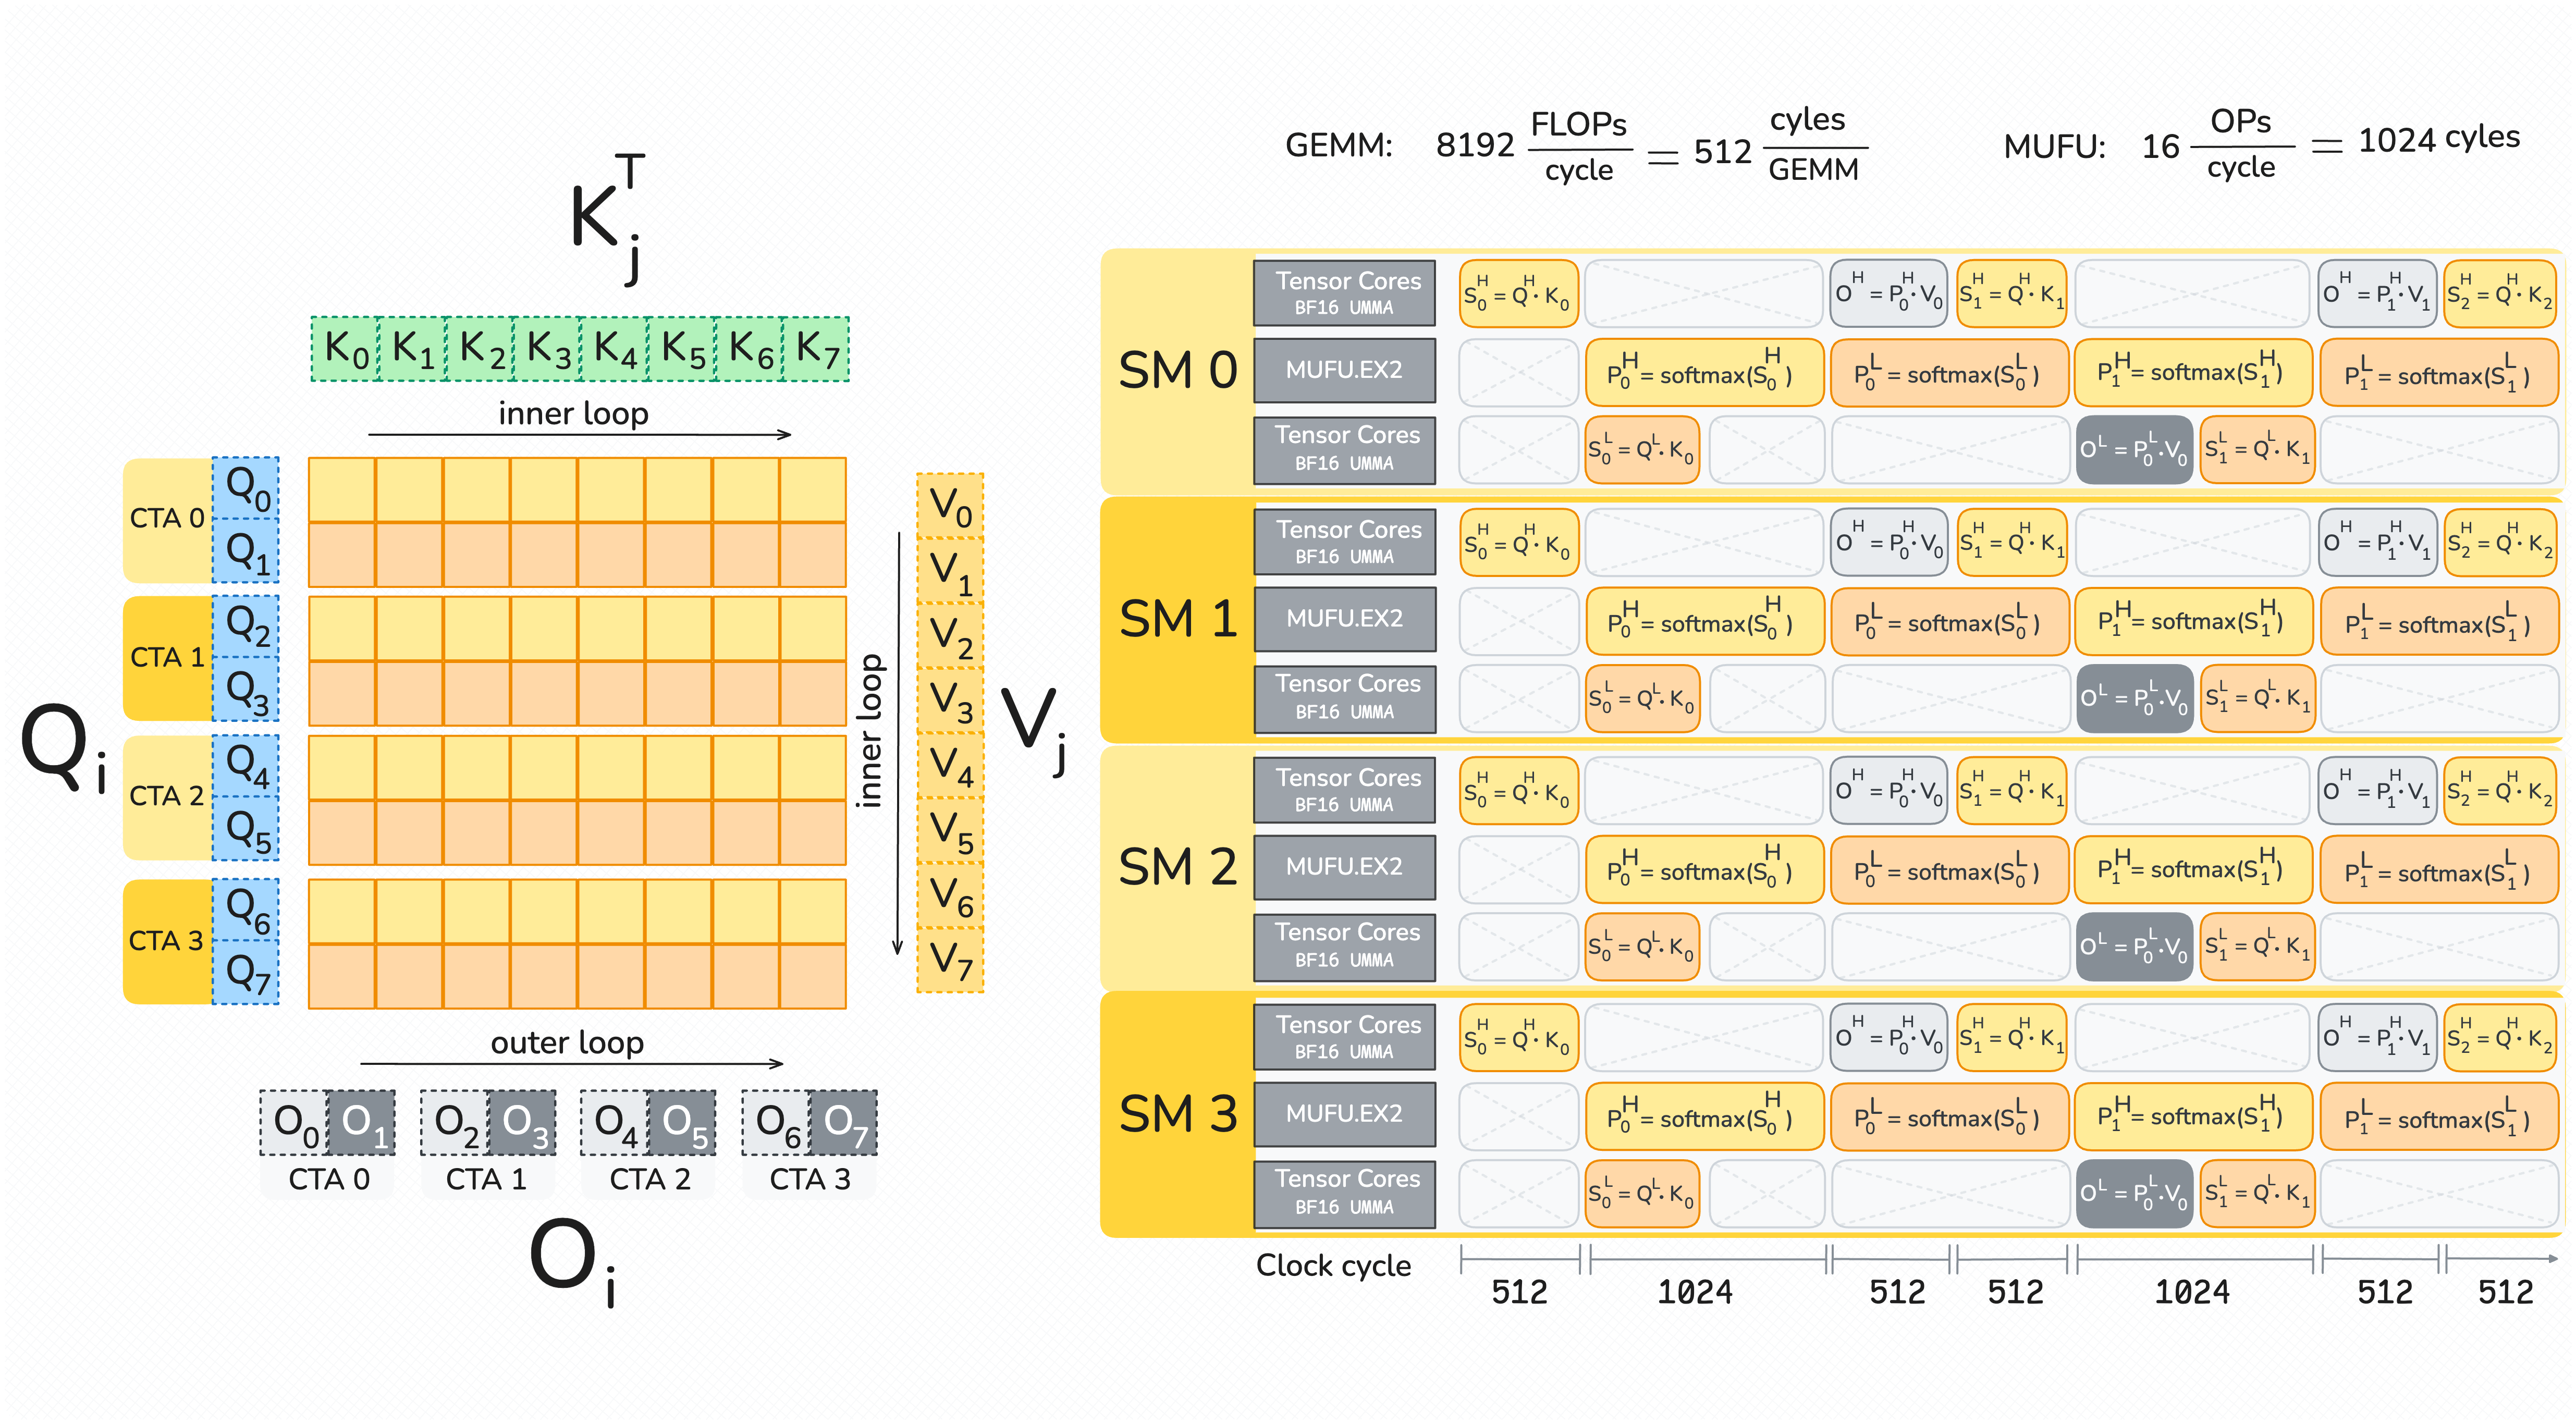
\includegraphics[width=1.0\linewidth]{../Figures/FA4_FWD_p3.png}
  \caption{FlashAttention-4前向传播流水线。上标$^H$表示对应"高"Q块的矩阵，上标$^L$表示对应"低"Q块的矩阵。每个Q块对应128个查询token。}
  \label{fig:fwd_pipeline_wide}
\end{figure*}

\begin{table}[t]
\centering
\small
\begin{tabular}{lcc}
\toprule
资源 & $128^3$ & $256 \times 128^2$ \\
\midrule
MMA计算 & \textbf{1024} & \textbf{2048} \\
共享内存 & 768 & 1536 \\
指数运算单元 & \textbf{1024} & \textbf{2048} \\
\bottomrule
\end{tabular}
\caption{注意力前向传播的屋顶线分析（单位：周期）。对于两种分块尺寸，MMA计算和指数运算单元均为主要瓶颈。}
\label{tab:fwd_roofline}
\end{table}

\subsubsection{重叠矩阵乘法与softmax的新流水线}

由于Blackwell架构再次将张量核心FLOPS翻倍，注意softmax与张量核心操作的重叠比在Hopper上更为关键。我们遵循类似FA-3的乒乓调度方式，每个线程块计算两块输出。
当一块的张量核心操作执行时，另一块计算softmax。
Hopper张量核心以交错模式将累加器保存在寄存器中（每行四个线程），而Blackwell张量核心将累加器保存在张量内存中。
此外，Blackwell上单个累加器块为128 × 128个元素，而Hopper的块大小为64 × 128。

在这些块上分配工作的自然方式是使用两组128个线程的线程束组，每个线程处理整行。
这消除了用于规约行最大值的线程束间洗牌操作，以及每个线程的多个统计寄存器的需求。
与FA-3一样，我们显式同步两个softmax线程束组，使其在关键区（即指数计算部分）不重叠。
每个softmax线程束组首先将整行加载到寄存器，然后计算最大值，再计算softmax（即减去最大值、重缩放、指数化、转换为输入精度），最后计算行和。

与FA-3的另一个区别是，由于我们通过张量内存而非寄存器文件传输$\vP$，我们可以将输出的重缩放解耦到独立的"校正"线程束组，从而将其从关键路径中移除。

为实现这种流水线重叠，可以选择多种张量内存分区方案。所有方案都必须为两块输出分配空间，在头维度为128时，留下一半张量内存存储$\vS$和$\vP$。这些内存可以存储两个$\vS$副本或四个$\vP$副本（假设输入为FP16或BF16张量核心）。
这给我们留下了大致两种分区选项：一块$\vS$和两块$\vP$，或两块$\vS$与$\vP$重叠。我们选择后者，因为它允许我们立即从计算两块$\vS$开始软件流水线。这也留下了一些张量内存用于向校正线程束组传递重缩放统计信息。

较大的Blackwell分块尺寸和所选的线程分配方案引入了一个问题：除非从张量内存重新加载，否则我们必须在寄存器中保存整行的128个元素。
由于我们使用两个softmax线程束组、一个校正线程束组和一个驱动张量核心及TMA单元的线程束组，为softmax分配足够的寄存器并防止寄存器溢出至关重要。
对于BF16输入数据类型，我们需要128个寄存器存储输入，可能还需要64个寄存器存储输出（加上杂项和临时寄存器）。
为降低寄存器压力，我们分阶段存储$\vP$：前四分之三存储一次（并触发相应的MMA操作），最后四分之一单独存储。

\subsubsection{指数函数的软件模拟}

\textbf{指数运算吞吐量瓶颈。}
在现代GPU上，指数函数由多功能单元（MUFU）计算，其吞吐量远低于用于矩阵乘法的张量核心。在B200和GB200 GPU上，MUFU每时钟每SM提供16次操作，而矩阵乘法为每时钟每SM 8192次操作。由于softmax计算需要大量指数求值，这种差异使指数函数成为注意力内核中的关键瓶颈。

\textbf{通过多项式近似进行软件模拟。}
为提高指数运算吞吐量，我们使用浮点FMA单元实现了$2^x$的软件模拟，FMA单元可与MUFU并行运行。我们使用经典的范围归约技术（Cody-Waite方法）和多项式近似~\citep{muller2018handbook}。关键思路是分解指数计算：
{\setlength{\abovedisplayskip}{2pt}%
 \setlength{\belowdisplayskip}{2pt}%
 \setlength{\abovedisplayshortskip}{3pt}%
 \setlength{\belowdisplayshortskip}{3pt}%
\begin{equation}
2^x = 2^{\lfloor x \rfloor}\,2^{x-\lfloor x \rfloor}
\end{equation}}
其中$\lfloor x \rfloor$是整数部分，$x - \lfloor x \rfloor \in [0, 1)$是小数部分。

整数部分$2^{\lfloor x \rfloor}$可以利用IEEE 754浮点表示的位操作高效计算。由于指数字段直接表示2的幂次，计算$2^{\lfloor x \rfloor}$等价于对指数位进行移位和加法操作，这可以使用整数ALU指令完成。

对于小数部分，我们用多项式近似$2^{x_{\text{frac}}}$，其中$x_{\text{frac}} \in [0, 1)$：
\begin{equation}
2^{x_{\text{frac}}} \approx \sum_{i=0}^{n} p_i\, x_{\text{frac}}^i
\end{equation}
其中$p_0 = 1.0$，其余系数选取为在$[0, 1)$上最小化相对近似误差，使用Sollya软件包~\citep{chevillard2010sollya}计算。多项式求值使用Horner方法结合FMA指令，实现高吞吐量。

完整算法流程如下：
\begin{enumerate}
\item 将$x$截断至至少$-127$以避免下溢
\item 使用向下舍入模式计算$\lfloor x \rfloor$：将$2^{23} + 2^{22}$加到$x$上（将小数位强制到尾数中），然后以向下舍入模式减去
\item 计算小数部分：$x_{\text{frac}} = x - \lfloor x \rfloor$
\item 求多项式得$2^{x_{\text{frac}}}$
\item 合并整数和小数部分：将$\lfloor x \rfloor$移入指数字段并加上$2^{x_{\text{frac}}}$的尾数位
\end{enumerate}

通过将指数计算分布在MUFU和FMA单元上，这种方法有效提高了指数运算吞吐量，缓解了注意力计算中的关键瓶颈。

\textbf{部分模拟。}
尽管多项式模拟提高了指数运算吞吐量，但它有一定代价：更多寄存器（用于保存中间值和系数）、更高的寄存器带宽消耗以及比MUFU指令更长的延迟。对所有指数求值使用模拟会增加寄存器压力并可能导致溢出，从而抵消吞吐量提升。相反，我们只对每个softmax行中的一部分元素（10--25\%）应用模拟，其余通过硬件\texttt{MUFU.EX2}计算。确切比例根据给定分块配置下MMA和指数运算吞吐量的比率经验调优。

\textbf{数值精度。}
表~\ref{tab:ex2_accuracy}比较了不同次数的多项式近似与硬件\texttt{MUFU.EX2}指令的精度，在$[0, 1)$中的400万个随机输入上进行测量。我们报告两个指标：FP32级别的误差（量化前）和BF16级别的误差（将FP32输出舍入到BF16后），均相对于FP64参考值测量。

在FP32级别，3次多项式的最大相对误差为$8.8 \times 10^{-5}$，大约是硬件的600倍。然而，舍入到BF16后，误差变得几乎无法区分：BF16的量化误差（${\sim}3.9 \times 10^{-3}$）对所有$\geq 3$次多项式的近似误差均占主导地位。3次多项式在99\%的输入上与硬件结果相差1个BF16 ULP以内，这对于注意力计算已经足够，因为softmax输出以BF16精度被消耗。
更高次多项式可以缩小FP32差距：5次多项式在最大相对误差上与硬件相差不到2倍，代价是每次求值额外增加两条FMA指令。

\begin{table}[t]
\centering
\small
\begin{tabular}{lccccc}
\toprule
& \multicolumn{2}{c}{FP32 vs FP64} & \multicolumn{2}{c}{BF16 vs FP64} \\
\cmidrule(lr){2-3} \cmidrule(lr){4-5}
方法 & 最大相对误差 & 平均相对误差 & 最大相对误差 & 平均相对误差 \\
\midrule
理想（FP64$\to$BF16）& --- & --- & $3.89 \times 10^{-3}$ & $1.41 \times 10^{-3}$ \\
硬件 \texttt{MUFU.EX2} & $1.41 \times 10^{-7}$ & $3.04 \times 10^{-8}$ & $3.89 \times 10^{-3}$ & $1.41 \times 10^{-3}$ \\
3次多项式 & $8.77 \times 10^{-5}$ & $5.43 \times 10^{-5}$ & $3.90 \times 10^{-3}$ & $1.41 \times 10^{-3}$ \\
4次多项式 & $3.05 \times 10^{-6}$ & $1.84 \times 10^{-6}$ & $3.89 \times 10^{-3}$ & $1.41 \times 10^{-3}$ \\
5次多项式 & $1.44 \times 10^{-7}$ & $5.48 \times 10^{-8}$ & $3.89 \times 10^{-3}$ & $1.41 \times 10^{-3}$ \\
\bottomrule
\end{tabular}
\caption{在$[0, 1)$上$2^x$多项式模拟的精度，在400万个随机输入上相对FP64参考值测量。FP32列测量原始多项式输出；BF16列测量舍入到BF16后的结果。对于所有$\geq 3$次多项式，BF16量化误差占主导地位。}
\label{tab:ex2_accuracy}
\end{table}

\subsubsection{跳过在线softmax重缩放}

\textbf{FlashAttention在线softmax。}
FlashAttention分块计算注意力$\softmax(QK^\top)V$以最小化内存流量。为了数值稳定性，算法在处理各块时维护运行统计信息。计算第$j$块时，令$S_j = Q K_j^\top$为该块的注意力分数。在线softmax算法跟踪：
\begin{align*}
m_j &= \max(m_{j-1}, \rowmax(S_j)) \\
\ell_j &= e^{m_{j-1} - m_j} \ell_{j-1} + \rowsum(e^{S_j - m_j})
\end{align*}
其中$m_j$是运行最大值，$\ell_j$是指数的运行和（归一化因子）。中间输出$O_j$更新为：
$
O_j = e^{m_{j-1} - m_j} O_{j-1} + e^{S_j - m_j} V_j.
$
重缩放因子$e^{m_{j-1} - m_j}$通过在遇到更大值时重新归一化之前的结果来确保数值稳定性。

\textbf{条件式重缩放。}
步骤$e^{m_{j-1} - m_j} O_{j-1}$需要一次向量乘法。我们做两个简单的观察：
\begin{enumerate}
\item 只有当$m_j > m_{j-1}$时（即发现新的更大值时）才需要重缩放。
\item 我们可以在重缩放上容忍一些"余量"：只有当$m_j - m_{j-1} > \tau$时才重缩放，其中$\tau$是一个阈值（通常设为$\log_2(256) = 8.0$，对应于256.0的重缩放因子）。只要我们跟踪统计信息（已执行的总缩放量），在最终仍可得到正确的分母以获得正确的最终输出。
\end{enumerate}

在\faf中，我们将算法修改为：
\begin{equation}
O_j = \begin{cases}
e^{m_{j-1} - m_j} O_{j-1} + e^{S_j - m_j} V_j & \text{若 } m_j - m_{j-1} > \tau \\
O_{j-1} + e^{S_j - m_{j-1}} V_j & \text{否则}
\end{cases}
\end{equation}
当$m_j - m_{j-1} \leq \tau$时，我们跳过更新$m$并继续使用$m_{j-1}$。这保持了正确性，因为在计算结束时，所有累积值均通过真实最大值$m_{\text{final}}$和最终归一化因子$\ell_{\text{final}}$重新归一化：
{\setlength{\abovedisplayskip}{0.1pt}%
 \setlength{\belowdisplayskip}{1pt}%
 \setlength{\abovedisplayshortskip}{0.1pt}%
 \setlength{\belowdisplayshortskip}{1pt}%
\begin{equation*}
\text{输出} = \frac{1}{\ell_{\text{final}}} O_{\text{final}}
\end{equation*}}
这一修改在保持数值精度的同时显著减少了重缩放操作的次数，因为最终归一化步骤会纠正跳过中间重缩放引入的小偏差。

实践中，为避免线程束分歧，当线程束中任何线程需要重缩放时，我们对整个线程束执行重缩放。
